% Render: pdflatex gambar-daerah-ptldv.tex
\documentclass[tikz]{standalone}
\usepackage{amsmath}
\definecolor{bg}{HTML}{171D2B}
\definecolor{aksen}{HTML}{F7B538}
\definecolor{hijau}{HTML}{4ADE80}
\definecolor{merah}{HTML}{F87171}
\begin{document}
\pagecolor{bg}
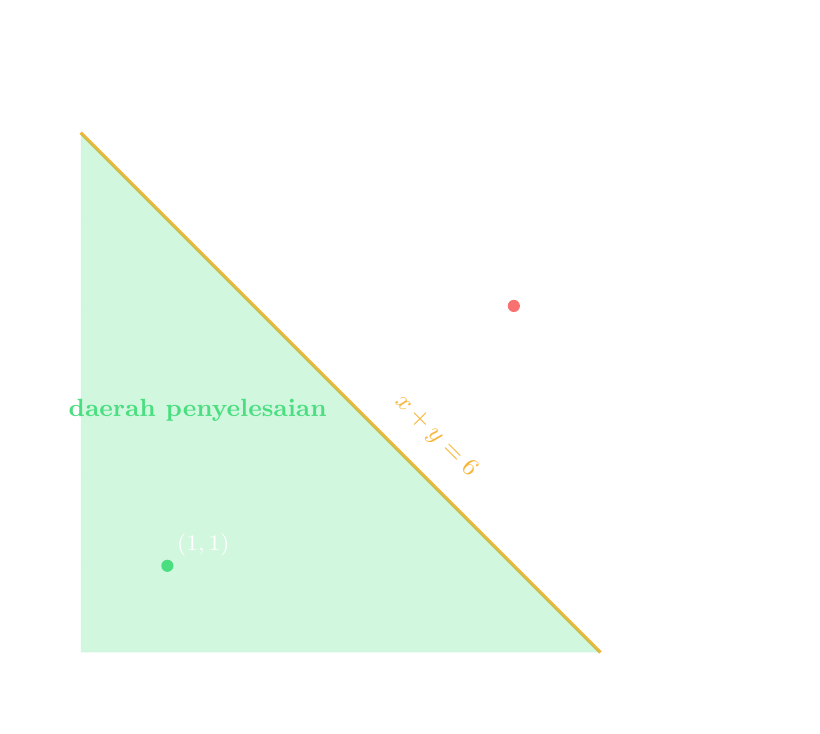
\begin{tikzpicture}[x=1.1cm, y=1.1cm, >=stealth]
  % Sumbu
  \draw[->, white, thick] (-0.6,0) -- (8.2,0) node[below left, white] {$x$};
  \draw[->, white, thick] (0,-0.6) -- (0,7.2) node[below left, white] {$y$};
  \foreach \i in {1,...,7} \draw[white!60] (\i,0.06) -- (\i,-0.06) node[below, white, font=\footnotesize] {$\i$};
  \foreach \j in {1,...,6} \draw[white!60] (0.06,\j) -- (-0.06,\j) node[left, white, font=\footnotesize] {$\j$};

  % Garis batas x + y = 6 (digambar dari (0,6) ke (6,0))
  \draw[aksen, very thick] (0,6) -- (6,0);

  % Daerah penyelesaian x + y <= 6 dengan x>=0, y>=0
  \fill[hijau, opacity=0.25] (0,0) -- (6,0) -- (0,6) -- cycle;

  % Titik-titik uji
  \fill[hijau] (1,1) circle (2.2pt) node[above right, white, font=\footnotesize] {$(1,1)$};
  \fill[merah] (5,4) circle (2.2pt) node[above right, white, font=\footnotesize] {$(5,4)$};

  % Label garis
  \node[aksen, font=\small, rotate=-45] at (4.1,2.5) {$x+y=6$};
  \node[hijau, font=\small\bfseries] at (1.35,2.8) {daerah penyelesaian};
\end{tikzpicture}
\end{document}
